\documentclass{article}
% PACKAGES
\usepackage[english]{babel}
\usepackage{graphicx} % Required for inserting images
\usepackage{lmodern}
\usepackage{tcolorbox}
\usepackage{amsmath}
\usepackage{pgfplots}
\usepackage{xcolor}
\usepackage{tikz}
\usepackage{color,soul}
\usepackage{enumerate}
\usepackage{enumitem}
\usepackage{cancel}
\usepackage{hyperref} 
\usepackage{tikzsymbols}
\usepackage{fontawesome5}
\usepackage[export]{adjustbox}
\usepackage{amssymb}



% COLOURS
\definecolor{Orchid}{RGB}{218, 112, 214}
\definecolor{snow}{rgb}{1.0, 0.98, 0.98}
\definecolor{mordantred19}{rgb}{0.68, 0.05, 0.0}
\definecolor{mistyrose}{rgb}{1.0, 0.89, 0.88}
\definecolor{nadeshikopink}{rgb}{0.96, 0.68, 0.78}
\definecolor{cadmiumgreen}{rgb}{0.0, 0.42, 0.24}


\title{MCV4U - Calculus}
\author{Kensukeken}
\date{30 January 2024}

\begin{document}
\maketitle

\tableofcontents
\newpage




\subsection{Introduction}
\textbf{What is Calculus?}\\
Two simple geometric problems originally led to the development of what is now called calculus. Both problems can be stated in terms of the graph of a function $y=f(x)$.
\begin{itemize}
    \item The problem of tangents: What is the slope of the tangent to the graph of a function at a given point P?
    \item The problem of areas: What is the area under a graph of a function $y=f(x)$ between $x=a$ and $x=b$.
\end{itemize}
    \begin{figure}[ht]
    \centering
    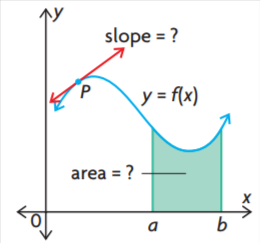
\includegraphics[width=0.35\textwidth]{imgs/Chapter 1 - MCV4U Nelson.png}
    \end{figure}
Isaac Barrow, a professor at the University of Cambridge, recognized the connection between the problem of tangents and the problem of areas. Newton and Gottfried Wilhelm von Leibniz independently solved these problems using differentiation and integration, a major advance in mathematics. This discovery led to the creation of calculus, a powerful branch of mathematics used in applied mathematics, science, engineering, and economics. The study of calculus begins with the meaning of a tangent, rate of change, limits, and the derivative of a function.
\newpage

\subsection*{Radical Expressions: Rationalizing Denominators}
In calculus, rationalizing the denominator of radical expressions involves simplifying expressions with radicals in the denominator. This process simplifies numbers into integers, making dividing by an integer more preferable than dividing by a radical number. \\ 

\subsection*{\textcolor{blue}{Selecting a strategy to rationalize the denominator}}
\begin{align*}
&\text{Simplify the radical expression } \frac{5}{2 \sqrt{6}+3} \text{ by rationalizing the denominator.} \\
&\text{Solution} \\
&\frac{5}{2 \sqrt{6}+3} = \frac{5}{2 \sqrt{6}+3} \times \frac{2 \sqrt{6}-3}{2 \sqrt{6}-3} \quad \text{(The conjugate $2 \sqrt{6}+\sqrt{3}$ is $2 \sqrt{6}-\sqrt{3}$)} \\
&= \frac{5(2 \sqrt{6}-3)}{4 \sqrt{36}-9} \\
&= \frac{5(2 \sqrt{6}-3)}{24-9} \\
&= \frac{5(2 \sqrt{6}-3)}{15} \\
&\text{(Divide by the common factor of 5)} \\
&= \frac{2 \sqrt{6}-3}{3}
\end{align*}
\\\\
When the denominator of a radical fraction is a two-term expression, you can rationalize the denominator by multiplying by the \textbf{\textcolor{blue}{conjugate}}. \\ \\
An expression such as $\sqrt{a}+\sqrt{b}$ has $\sqrt{a}-\sqrt{b}$ the conjugate.\\\\
Why are conjugates important? Recall that the linear terms are eliminated when
expanding a difference of squares. For example,
\begin{align*}
    (a-b)(a+b)&=a^2+ab-ab-b^2 \\
    &=a^2-b^2
\end{align*}
If a and b were radicals, squaring them would rationalize them.
\begin{align*}
\text{Consider this product:}\quad
    &(\sqrt{x}-\sqrt{y})(\sqrt{x}+\sqrt{y}), \; x, \text{y rational} \\ &=(\sqrt{x})^2+\sqrt{xy}-\sqrt{xy}-(\sqrt{x})^2 \\
    &=x-y \quad \textbf{Notice that the result is rational!}
\end{align*}

\newpage
\section{Unit 1 - Limits}
\subsection{Evaluating Limits Graphically}
Imagine someone is standing 10 metres from a wall. We tell that person to move halfway to the wall. We then them to again move halfway to the wall. We then tell them to again move halfway to the wall, and we continue to do this. Theoretically, the person will never reach the wall. However, we can say that as the number of trials moves to infinity, the limit of where the person is standing will be the wall.

Of course, the person will never each the wall(theoretically), but we could still refer to the wall as the limit.

Another way to think about limits is to think about sequnces.

Consider the sequence $f(n)$ where n is a positive integer referring to the ordinal position of the term in the sequence and $f(n)$ is the value of that term.
$$1,\frac{1}{2},\frac{1}{4},\frac{1}{8},\frac{1}{16}, \cdots $$
The values are getting closer and closer to 0. We know that the values will never reach 0, but they will get infinitely close to 0. We can say that the limit of the sequence as the number of terms goes to infinity is 0.

$$\lim_{n \to \infty} f(n)=0$$
In mathematics, a limit is the value that a function(or sequence) "approaches" as the input (or index) "approaches" some value. Limits are essential to calculus(and mathematical analysis in general) and are used to define continuity, derivatives, and integrals.When dealing with functions, we can let the x-value inputted to the function grow closer and closer to some set value. We then watch the pattern of y-values to see if there is a set y-value that we grow infinitely close to. If there is such a value, we say that that is the value of the limit

\subsubsection{Example:}
Suppose that we wish to determine $\lim_{x \to 3} (-x^2+6x-5 )$. We can draw the graph of $y=-x^2+6x-5$:

\begin{minipage}{0.6\textwidth}
    \begin{align*}
        \lim_{x \to 3^-} f(x) &= 4 \\
        \lim_{x \to 3^+} f(x) &= 4 \\
        \lim_{x \to 3} f(x) &= 4
    \end{align*}
\end{minipage}%
\vspace{0.1em}%
\begin{minipage}{0.6\textwidth}
    The graph of $y=-x^2+6x-5$:
    \begin{center}
        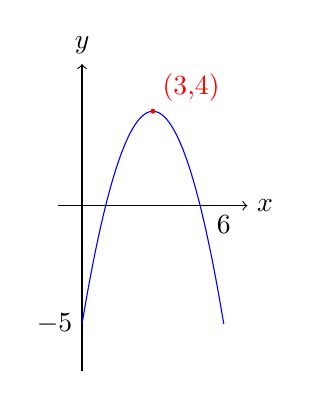
\begin{tikzpicture}[scale=0.3]
            % Axis
            \draw[->] (-1,0) -- (7,0) node[right] {$x$};
            \draw[->] (0,-7) -- (0,6) node[above] {$y$};
          
            % Function plot
            \draw[domain=0:6, smooth, variable=\x, blue] plot ({\x}, {-\x^2 + 6*\x - 5});
            \fill[red] (3, 4) circle (3pt) node[above right] {(3,4)};

          
            % Labels
            \node[below] at (6,0) {$6$};
            \node[left] at (0,-5) {$-5$};
        \end{tikzpicture}
    \end{center}
\end{minipage}
When determining whether the limit as x approaches a particular value of a function exists, we compare the two one-sided limits and see if they are the same. If they are, then the limit exists, and is equal to that common value.
\\ 
\begin{tcolorbox}[colback=Orchid!5!white,colframe=cadmiumgreen!75!white,coltitle=white,]
If $\lim _{x \rightarrow a^{-}} f(x)=b$ and if $\lim _{x \rightarrow a^{+}} f(x)=b$ then $\lim _{x \rightarrow a} f(x)=b$
However, if $\lim _{x \rightarrow a^{-}} f(x)$ exists and if $\lim _{x \rightarrow a^{+}} f(x)$ exists but $\lim _{x \rightarrow a^{-}} f(x) \neq \lim _{x \rightarrow a^{+}} f(x)$, then $\lim _{x \rightarrow a} f(x)$ does not exist. \\ \\ 
\end{tcolorbox}

Note that in the last example, we expressed that limits were described as being equal to $\infty$ and to $-\infty$. Technically, nothing can be equal to $\infty$ or $-\infty$, so one could immediately conclude that $\lim_{x \to 4}\left( \frac{x+1}{x-4}\right)$ does not exist, as soon as one of the one-sided limits is equal to $\infty$ or $-\infty$. However, in this course, we will allow one-sided limits to be expressed as $\infty$ or $-\infty$. This will include limits as $x$ approaches $\infty$ or $-\infty$, which can only be approached from one direction. 

However, if we are seeking the limit of a function as $x$ approaches a real number (a two-sided limit), and if one of the one-sided limits is equal to $\infty$ or $-\infty$, then we will state that the limit of the function as $x$ approaches the real number does not exist.
\\
\subsubsection*{Limits that can only be approached from one side:}
Sometimes, we will come across a limit that can only be approached from the left or from the right. The most common type of limit of this form is when we seek to find the limit of a function as $x$ approaches $\infty$ or as $x$ approaches $-\infty$.

If we want to evaluate the limit of a function as $x$ approaches $-\infty$, we can only approach it from the right because we can’t be to the left of $-\infty$. Similarly, if we want to evaluate the limit of a function as $x$ approaches $\infty$, we can only approach it from the left because we can’t be to the right of $\infty$.

\begin{table}[h]
    \centering
    \begin{tabular}{|c|l|}
    \hline
    Expression & Explanation \\
    \hline
    $\frac{0}{0}$ & Indeterminate: maybe the limit and maybe it doesn't. Do more work! \\
    \hline
    $\frac{\text{Non-Zero}}{0}$ & The limit does not exist. You're done working. \\
    \hline 
    $\frac{\text{Anything}}{\text{Non-Zero}}$ & That's the answer :) \\
    \hline
    \end{tabular}
    \caption{Limit Evaluation Cases}
    \label{tab:limits}
\end{table}

\newpage

\subsection{Evaluating Limits Algebraically}
Assume that we are trying to evaluate $\lim_{x \to c}f(x), c \in \mathrm{R}$\\

We often don't use a graphing approach to evaluate a limit. Rather, we can use an algebraic approach if we remember the following steps. \\
\begin{enumerate}
    \item  \text{\hl{If the curve is continuous at $\mathrm{x}=\mathrm{c}$}}, then we can simply evaluate $\mathrm{f}(\mathrm{c})$. In other words, $\lim _{x \rightarrow c} f(x)=f(c)$ \\
    \begin{itemize}
        \item This happened in the first example in the powerpoint about evaluating limits graphically. When we were seeking to evaluate $\lim _{x \rightarrow 3}\left(-x^2+6 x-5\right)$, we could have recognized that this was a continuous function at $x=3$ and simply plugged in an $x$-value of 3 .
   \end{itemize}
\item \hl{However, sometimes direct substitution leads to a result of $0 / 0$.} Obviously, this result is undefined. However, the limit may still exist because there may be a hole at $\mathrm{x}=\mathrm{c}$ in an otherwise continuous curve.
\begin{itemize}
    \item This is what happened in some of our examples in the powerpoint on graphically evaluating limits. For example, in the example where we sought $\lim _{x \rightarrow-2}\left(\frac{x^2+3 x+2}{x+2}\right)$, there was a hole and the value of the limit equaled the $y$-coordinate of the location of the hole.
\end{itemize} 
When we get the indeterminate form of $0 / 0$, we can try the following:
\begin{tcolorbox}[colback=Orchid!5!white,colframe=Orchid!75!white,coltitle=white,]
\begin{enumerate}[label=(\roman*)]
    \item Factor numerator and denominator, and the offending factor may cancel out of both
    \item Rationalize the numerator and/or denominator and see if this leads you to be able to directly substitute
    \item Simplify the function prior to substituting to see if that allows you to directly substitute iv. Introduce a new factor that allows the numerator and/or denominator to become a difference or sum of nth powers, which then creates the offending factor which can then be canceled from both numerator and denominator (you may wish to introduce a new variable to do this)
\end{enumerate}
\end{tcolorbox}
\end{enumerate}
\newpage

\subsubsection{Examples where direct substitution leads to the correct answer}
\textbf{Examples}\\
1. Evaluate $\lim_{x \to 5}x^2+2x-3$
\begin{align*}
\lim_{x \to 5}x^2+2x-3 &= \text{Plug } x=5 \\ 
    &= (5)^2+2(5)-3 \\
    &= \boxed{32} \quad \text{That's the answer } 
\end{align*}
2. Evaluate $\lim_{x \to 3}\frac{\sqrt{x-1}-\sqrt{x+1}}{\sqrt{x-3}-\sqrt{x+3}}$\\
\begin{align*}
    &=\frac{\sqrt{3-1}-\sqrt{3+1}}{\sqrt{3-3}-\sqrt{3+3}}\\
    &=\frac{\sqrt{2}-\sqrt{4}}{\sqrt{0}-\sqrt{6}}\\
    &=\frac{\sqrt{2}-2}{-\sqrt{6}}
\end{align*}

2a)  Examples where Direct Substitution Leads to 0/0 But you can then factor, cross out, and then sub in\\\\
3. Evaluate $\lim_{h \to 0}\frac{(2+h)^3-8}{h}$
\begin{align*}
    &\text{Recall}: a^3-b^3 = (a-b)(a^2+ab+b^2)\\
    &=\lim_{h\to 0}\frac{\cancel{8}+12h^+6h^2+h^2\cancel{-8}}{h}\\
    &=\lim_{h\to 0}\frac{h^3+6h^2+12}{h}\\
    &=\lim_{h \to 0}\frac{\cancel{h}(h^2+6h+12)}{\cancel{h}}\\
    &= (0)^2+6(0)+12\\
    &=12
\end{align*}
4. Evaluate $\lim_{x \to 25}\frac{x-25}{\sqrt{x}-5}$
\begin{align*}
    &=\lim_{x \to 25}\frac{x-25}{\sqrt{x}-5} \times \frac{(\sqrt{x})^2-(5)^2}{\sqrt{x}-5}\\
    &=\lim_{x \to 25}\frac{\cancel{(\sqrt{x}-5)}(\sqrt{x}+5)}{\cancel{(\sqrt{x}-5)}}\\
    &=\sqrt{25}+5\\
    &=10
\end{align*}
\subsubsection{Difference of nth Powers Factoring}

The formula for factoring the difference of nth powers is:

\[
a^n - b^n = (a - b)(a^{n-1} + a^{n-2}b + a^{n-3}ba^2 + \cdots + ab^{n-2} + b^{n-1})
\]

Examples of the difference of nth powers factored from \(a^2 - b^2\) to \(a^{10} - b^{10}\) using the formula:

\begin{enumerate}
    \item \(a^2 - b^2\):
    \[
    a^2 - b^2 = (a - b)(a + b)
    \]
    
    \item \(a^3 - b^3\):
    \[
    a^3 - b^3 = (a - b)(a^2 + ab + b^2)
    \]
    
    \item \(a^4 - b^4\):
    \[
    a^4 - b^4 = (a - b)(a^3 + a^2b + ab^2 + b^3)
    \]
    
    \item \(a^5 - b^5\):
    \[
    a^5 - b^5 = (a - b)(a^4 + a^3b + a^2b^2 + ab^3 + b^4)
    \]
    
    \item \(a^6 - b^6\):
    \[
    a^6 - b^6 = (a - b)(a^5 + a^4b + a^3b^2 + a^2b^3 + ab^4 + b^5)
    \]
    
    \item \(a^7 - b^7\):
    \[
    a^7 - b^7 = (a - b)(a^6 + a^5b + a^4b^2 + a^3b^3 + a^2b^4 + ab^5 + b^6)
    \]
    
    \item \(a^8 - b^8\):
    \[
    a^8 - b^8 = (a - b)(a^7 + a^6b + a^5b^2 + a^4b^3 + a^3b^4 + a^2b^5 + ab^6 + b^7)
    \]
    
    \item \(a^9 - b^9\):
    \[
    a^9 - b^9 = (a - b)(a^8 + a^7b + a^6b^2 + a^5b^3 + a^4b^4 + a^3b^5 + a^2b^6 + ab^7 + b^8)
    \]
    
    \item \(a^{10} - b^{10}\):
    \[
    a^{10} - b^{10} = (a - b)(a^9 + a^8b + a^7b^2 + a^6b^3 + a^5b^4 + a^4b^5 + a^3b^6 + a^2b^7 + ab^8 + b^9)
    \]
\end{enumerate}

These examples demonstrate the application of the difference of nth powers factoring formula for various powers from 2 to 10.

\subsection*{Sum of nth Powers Factoring (for odd n)}

If \( n \) is an odd positive integer, the sum of nth powers can be factored as follows:

\[
a^n + b^n = (a + b)(a^{n-1} - a^{n-2}b + a^{n-3}b^2 - \cdots - ab^{n-2} + b^{n-1})
\]

This formula works only when \( n \) is an odd positive integer.

\subsection*{Examples}

Let's consider the following examples:

\begin{enumerate}
    \item For \( n = 2 \):
    \[
    a^2 + b^2 \quad \text{(This formula doesn't apply)}
    \]
    
    \item For \( n = 3 \):
    \[
    a^3 + b^3 = (a + b)(a^2 - ab + b^2)
    \]
    
    \item For \( n = 4 \):
    \[
    a^4 + b^4 \quad \text{(This formula doesn't apply)}
    \]
    
    \item For \( n = 5 \):
    \[
    a^5 + b^5 = (a + b)(a^4 - a^3b + a^2b^2 - ab^3 + b^4)
    \]
    
    \item For \( n = 6 \):
    \[
    a^6 + b^6 \quad \text{(This formula doesn't apply)}
    \]
    
    \item For \( n = 7 \):
    \[
    a^7 + b^7 = (a + b)(a^6 - a^5b + a^4b^2 - a^3b^3 + a^2b^4 - ab^5 + b^6)
    \]
    
    \item For \( n = 8 \):
    \[
    a^8 + b^8 \quad \text{(This formula doesn't apply)}
    \]
    
    \item For \( n = 9 \):
    \[
    a^9 + b^9 = (a + b)(a^8 - a^7b + a^6b^2 - a^5b^3 + a^4b^4 - a^3b^5 + a^2b^6 - ab^7 + b^8)
    \]
    
    \item For \( n = 10 \):
    \[
    a^{10} + b^{10} \quad \text{(This formula doesn't apply)}
    \]
\end{enumerate}

These examples demonstrate the application of the formula for factoring the sum of nth powers when \( n \) is an odd positive integer.

\subsection*{Sum of nth powers factoring is really just an extension of difference of nth powers factoring.}
For example, consider $a^5+b^5$

$$
\begin{aligned}
& a^5+b^5 \\
& =a^5-(-b)^5 \\
& =[a-(-b)]\left[a^4+a^3(-b)+a^2(-b)^2+a(-b)^3+(-b)^4\right] \\
& =[a+b]\left[a^4+\left(-a^3 b\right)+a^2 b^2+\left(-a b^3\right)+b^4\right] \\
& =(a+b)\left(a^4-a^3 b+a^2 b^2-a b^3+b^4\right)
\end{aligned}
$$ 
\subsection*{Check Your Understanding:}
\begin{enumerate}
    \item Evaluate $\lim_{x \to 3}\frac{2x^4-162}{-x^5+243}$
    \item Evaluate $\lim_{x \to -2}\frac{x^7+128}{10x+20}$ 
\end{enumerate}
Feel free to download "chap 1.020.evaluating limits algebraically.pptx" to check the solutions in the "Lessons in PowerPoint Form" folder :) \\

 2b)  Examples where direct substitution leads to 0/0 but we can rationalize the numerator and/or denominator, then perhaps factor, then cross out then substitute\\

 1. Evaluate $\lim_{h\to 0}\frac{\sqrt{16+h}}{h}$
 \begin{align*}
     &=\lim_{h\to 0}\frac{(\sqrt{16+h}-4)(\sqrt{16-h}+4)}{h(\sqrt{16+h}+4)}\\
     &=\lim_{h\to 0}\frac{\cancel{16}+h\cancel{-16}}{h(\sqrt{16+h}+4)}\\
     &=\lim_{h\to 0}\frac{\cancel{h}}{\cancel{h}(\sqrt{16+h}+4)}\\
     &=\frac{1}{\sqrt{16+0}+4}\\
     &=\frac{1}{8}
 \end{align*}
2. Evaluate $\lim_{x \to 2}\frac{\frac{1}{x}-\frac{1}{2}}{x-2}$
\begin{align*}
    &=\lim_{x \to 2}\frac{\frac{2}{2x}-\frac{x}{2x}}{x-2}\\
    &=\lim_{x \to 2}\frac{\frac{2-x}{2x}}{x-2}\\
    &=\lim_{x \to 2}\frac{2-x}{2x(x-2)}\\
    &=\lim_{x \to 2}\frac{(-1)\cancel{(x-2)}}{(2x)\cancel{(x-2)}}\\
    &=-\frac{1}{4}
\end{align*}



2c) Examples where direct substitution leads to $\frac{0}{0}$, but we can create a difference of nth powers or sum of nth powers (if $n$ is odd) and then factor and cross out to substitute.

\textbf{**Some people find it beneficial to introduce a new variable in these questions, but it is not necessary.}\\\\
1. Evaluate $\lim_{x \to 64}\frac{\sqrt[3]{x}-4}{x-64}$
\begin{align*}
    & \text{Let }\quad a=x^\frac{1}{3}, \quad b=4\\
    &=\lim_{x \to 64}\frac{a-b}{x-64}\\
    &=\lim_{x \to 64}\frac{(a-b)(a^2+ab+b^2)}{(x-64)(a^2+ab+b^2)}\\
    &=\lim_{x \to 64}\frac{a^3-b^3}{(x^{\frac{2}{3}}+4x^{\frac{1}{4}}+16)}\\
    &=\lim_{x \to 64}\frac{\cancel{x-64}}{\cancel{(x-64)}(x^{\frac{2}{3}}+4x^{\frac{1}{4}}+16)}\\
    &=\frac{1}{(64)^{\frac{2}{3}}+4(64)^{\frac{1}{4}}+16)}\\
    &=\frac{1}{16+16+16}\\
    &=\frac{1}{48}
\end{align*}
\newpage
\subsection{One Sided Limits}
Recall this statement about limits from an earlier lesson.\\\\
If $\lim_{x\to a^-}f(x)=b$ and if $\lim_{x\to a^+}f(x)=b$ then $\lim_{x\to a}f(x)=b$.\\
However, if $\lim_{x \to a^{-}}f(x)$ exists and if $\lim_{x \to a^+}$ exists but $\lim_{x \to a^-}f(x)\neq \lim_{x \to a^+}f(x)$, then $\lim_{x \to a}f(x)$ does not exist.

\subsubsection*{Examples}
\begin{minipage}{0.35\textwidth}
    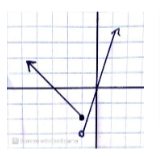
\includegraphics[width=\textwidth]{imgs/ex1.png}
\end{minipage}
\hspace{0.05\textwidth}
\begin{minipage}{0.6\textwidth}
    $\text{1. Given that}$
    $$f(x)=\left\{\begin{array}{c}
    -x-3, x \leq 1 \\
    3 x, x>-1
    \end{array}\right\},$$
    $\text{use a graphing approach to determine} \lim\limits_{x \to -1} f(x)$ or justify that it does not exist.
    $\lim_{x \to -1^-}f(x)=-2$\\
    $\lim_{x\ to -1^+}f(x)=-3$\\
   $\boxed{\therefore\ \lim\limits_{x \to -1} f(x)\text{ does not exist}}$
    \vspace{1cm}
\end{minipage}
Evaluate the following using a graphing approach:
\[
\lim_{x \to 2}\left(\sqrt{x-2}+3\right)
\]
\noindent
\begin{minipage}[t]{0.5\textwidth}
    \vspace{0pt}
    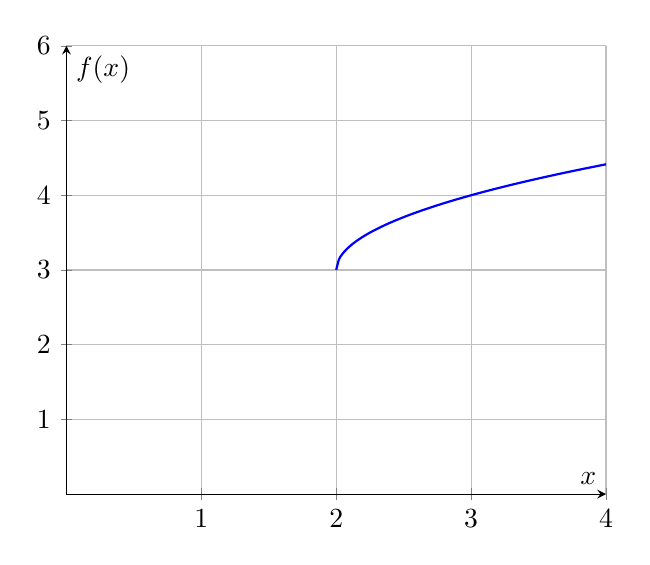
\begin{tikzpicture}
        \begin{axis}[
            xlabel=$x$,
            ylabel={$f(x)$},
            axis lines=middle,
            xmax=4,
            ymax=6,
            xmin=0,
            ymin=0,
            xtick={0,1,...,4},
            ytick={0,1,...,6},
            grid=both,
            domain=2:4,
            samples=100,
            smooth,
            legend pos=north west,
        ]
            \addplot[blue,thick] {sqrt(x-2) + 3};
        \end{axis}
    \end{tikzpicture}
\end{minipage}
\hfill
\begin{minipage}[t]{0.4\textwidth}
    \vspace{0pt}
    \begin{align*}
        \lim_{x \to 2^-}\left(\sqrt{x-2}+3\right) &= 3 \\
        \therefore \lim_{x \to 2}\left(\sqrt{x-2}+3\right) &= 3
    \end{align*}
\end{minipage}
\newpage 
\subsection{Limits as x goes to Negative infinity or Infinity}
We previously discussed how to evaluate limits as x goes to infinity or as x goes to negative infinity using a graphing approach.\\
However, we can discuss how to evaluate these types of limits without using a graphing approach every time.\\
To discuss how to do this, we will look at some graphs.
It is NOT important to know the numbers of the scenarios that follow.

\subsubsection{Scenario 1}
\begin{minipage}[t]{0.5\textwidth}
    \vspace{0pt}
    Suppose $y=a^x, 0 <a<1$\\
    For example, suppose $y=\left(\frac{1}{2}\right)^x$\\
    $\lim_{x \to -\infty}f(x)=\infty$\\
    $\lim_{x \to \infty}f(x)=0$
\end{minipage}
\begin{minipage}[t]{0.45\textwidth}
    \vspace{0pt}
    \begin{tikzpicture}[scale=0.8]
        \draw[->] (-3,0) -- (3,0) node[below] {$x$};
        \draw[->] (0,-1) -- (0,3) node[left] {$f(x)$};
        \draw[domain=-2:3,smooth,variable=\x,blue] plot ({\x},{0.5^\x});
        \draw[dashed] (-3,2) -- (3,2) node[right] {$1$};
        \draw[dashed] (-2,0) -- (-2,0.5) node[above] {$a$};
    \end{tikzpicture}
\end{minipage}

\subsubsection{Scenario 2}
\begin{minipage}[t]{0.5\textwidth}
    \vspace{0pt}
    Suppose $y=a^x, a>1$\\
    For example, suppose $y=2^x$\\
    $\lim_{x \to -\infty}f(x)=0$\\
    $\lim_{x \to \infty}f(x)=\infty$
\end{minipage}
\begin{minipage}[t]{0.45\textwidth}
    \vspace{0pt}
    \begin{tikzpicture}[scale=0.8]
        \draw[->] (-3,0) -- (3,0) node[below] {$x$};
        \draw[->] (0,-1) -- (0,3) node[left] {$f(x)$};
        \draw[domain=-2:2,smooth,variable=\x,blue] plot ({\x},{2^\x});
        \draw[dashed] (-3,1) -- (3,1) node[right] {$1$};
        \draw[dashed] (-2,0) -- (-2,2) node[above] {$a$};
    \end{tikzpicture}
\end{minipage}

\subsubsection{Scenario 3}
\begin{minipage}[t]{0.5\textwidth}
    \vspace{0pt}
    Suppose $y=a^x, a=1$\\
    $\lim_{x \to -\infty}f(x)=1$\\
    $\lim_{x \to \infty}f(x)=1$
\end{minipage}
\begin{minipage}[t]{0.45\textwidth}
    \vspace{0pt}
    \begin{tikzpicture}[scale=0.8]
        \draw[->] (-3,0) -- (3,0) node[below] {$x$};
        \draw[->] (0,-1) -- (0,3) node[left] {$f(x)$};
        \draw[domain=-3:3,smooth,variable=\x,blue] plot ({\x},{1^\x});
        \draw[dashed] (-3,1) -- (3,1) node[right] {$1$};
        \draw[dashed] (-2,0) -- (-2,1) node[above] {$a$};
    \end{tikzpicture}
\end{minipage}

\subsubsection{Scenario 4}
\begin{minipage}[t]{0.5\textwidth}
    \vspace{0pt}
    Suppose $y=x^a, a>0$\\
    $\lim_{x \to \infty}f(x)=\infty$
\end{minipage}
\begin{minipage}[t]{0.45\textwidth}
    \vspace{0pt}
    \begin{tikzpicture}[scale=0.8]
        \draw[->] (0,0) -- (3,0) node[below] {$x$};
        \draw[->] (0,0) -- (0,3) node[left] {$f(x)$};
        \draw[domain=0.1:3,smooth,variable=\x,blue] plot ({\x},{\x});
        \draw[dashed] (0,0) -- (3,3) node[right] {$x^a$};
    \end{tikzpicture}
\end{minipage}

\subsubsection{Scenario 5}
\begin{minipage}[t]{0.5\textwidth}
    \vspace{0pt}
    Suppose $y=x^a, a<0$\\
    For example, suppose $y=x^{-1/2}$ or $y=-2$\\
    $\lim_{x \to \infty}x^a=0$
\end{minipage}
\begin{minipage}[t]{0.45\textwidth}
    \vspace{0pt}
    \begin{tikzpicture}[scale=0.8]
        \draw[->] (0,0) -- (3,0) node[below] {$x$};
        \draw[->] (0,0) -- (0,3) node[left] {$f(x)$};
        \draw[domain=0.3:3,smooth,variable=\x,blue] plot ({\x},{1/\x});
        \draw[dashed] (0,0) -- (3,0) node[right] {$x^a$};
    \end{tikzpicture}
\end{minipage}

\subsubsection{Scenario 6}
\begin{minipage}[t]{0.5\textwidth}
    \vspace{0pt}
    Suppose $y=a^x, a=0$\\
    $\lim_{x \to \infty}f(x)=1$
\end{minipage}
\begin{minipage}[t]{0.45\textwidth}
    \vspace{0pt}
    \begin{tikzpicture}[scale=0.8]
        \draw[->] (0,0) -- (3,0) node[below] {$x$};
        \draw[->] (0,0) -- (0,3) node[left] {$f(x)$};
        \draw[domain=0:3,smooth,variable=\x,blue] plot ({\x},{1});
        \draw[dashed] (0,1) -- (3,1) node[right] {$a^x$};
    \end{tikzpicture}
\end{minipage}

\newpage
\textbf{\underline{Limits of Rational Functions as \( x \) Approaches Infinity or Negative Infinity:}}

When evaluating the limit of a rational function as \( x \) approaches either infinity or negative infinity (i.e., a polynomial over another polynomial), the following approach can be employed:

\begin{enumerate}
    \item Determine the degrees of the numerator and denominator. Factor out \( x^n \) from both the numerator and denominator, where \( n \) is the greater or lesser of the two degrees. If both degrees are the same, \( n \) equals that degree. (Factor out the same term from both the numerator and denominator.) Cancel out like factors.
    
    \item Determine the limit of each term in the numerator and sum those limits. Determine the limit of each term in the denominator and sum those limits.
    \begin{enumerate}
        \item A numerator with a finite limit over a denominator growing without bound yields a limit of 0.
        
        \item A numerator with a finite limit over a denominator with a finite limit produces a limit equal to the quotient of those limits.
        
        \item A numerator with a finite limit over a denominator that tends to zero yields a limit of infinity or negative infinity.
        
        \item A numerator growing without bound over a denominator that's finite or tends to zero produces a limit of infinity or negative infinity.
        
        \item A numerator that tends to zero over a denominator that's finite or growing without bound yields a limit of 0.
    \end{enumerate}
\end{enumerate}
\subsection{Continuity}

The idea of continuity can be thought of informally as the idea of being able to draw a graph without lifting one’s pencil.\\
Three types of discontinuity are illustrated below.

\begin{figure}[h]
\centering
\begin{minipage}{0.3\textwidth}
\centering
\begin{tikzpicture}[scale=0.8]
  % Axes
  \draw[->] (-1.5,0) -- (1.5,0) node[right] {$x$};
  \draw[->] (0,-1.5) -- (0,1.5) node[above] {$y$};
  
  % Hole
  \draw[fill=white] (0.75,0.75) circle [radius=0.03];
  \draw[dashed] (0.75,0.75) circle [radius=0.03];
  
  % Labels
  \node[below right] at (0.75,0.75) {$\circ$ Hole};
\end{tikzpicture}
\caption*{Graph with a Hole}
\end{minipage}%
\hfill
\begin{minipage}{0.3\textwidth}
\centering
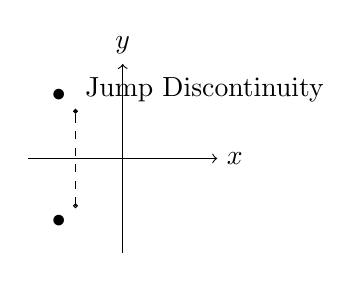
\begin{tikzpicture}[scale=0.8]
  % Axes
  \draw[->] (-1.5,0) -- (1.5,0) node[right] {$x$};
  \draw[->] (0,-1.5) -- (0,1.5) node[above] {$y$};
  
  % Jump Discontinuity
  \draw[fill=white] (-0.75,-0.75) circle [radius=0.03];
  \draw[fill=black] (-0.75,0.75) circle [radius=0.03];
  \draw[dashed] (-0.75,-0.75) -- (-0.75,0.75);
  
  % Labels
  \node[below left] at (-0.75,-0.75) {$\bullet$};
  \node[above left] at (-0.75,0.75) {$\bullet$};
  \node[above right] at (-0.75,0.75) {Jump Discontinuity};
\end{tikzpicture}
\caption*{Graph with a Jump Discontinuity}
\end{minipage}%
\hfill
\begin{minipage}{0.3\textwidth}
\centering
\begin{tikzpicture}[scale=0.8]
  % Axes
  \draw[->] (-1.5,0) -- (1.5,0) node[right] {$x$};
  \draw[->] (0,-1.5) -- (0,1.5) node[above] {$y$};
  
  % Vertical Asymptote
  \draw[dashed] (1,-1.5) -- (1,1.5);
  
  % Labels
  \node[above right] at (1,1.5) {Vertical Asymptote};
\end{tikzpicture}
\caption*{Graph with a Vertical Asymptote}
\end{minipage}
\end{figure}
\[
\boxed{\text{The function } f \text{ is continuous at } x=a \text{ if } f(a) \text{ is defined and if } f(a) = \lim_{x\to a} f(x)}
\]

\subsubsection{General Observations Regarding Continuity:}
\begin{enumerate}
    \item A function that is not continuous has some type of break in its graph.  This break is the result of a hole, jump, or vertical asymptote.
\item All polynomial functions are continuous for all real numbers.
\item A rational function $h(x)=\frac{f(x)}{g(x)}$is continuous at $x=a$ if $g(a)\neq 0$
\item A rational function in simplified for has a discontinuity at the zeros of the denominator.
\item When the one-sided limits are not equal to each other, then the limit at this point does not exist and the function is not continuous at this point
\end{enumerate}
\subsection{Properties of Limits}
\begin{itemize}
\item 1) $\lim _{x \rightarrow a} x=a$ \\
\item 2) $\lim _{x \rightarrow a} c=c$ \\
\item 3) $\lim _{x \rightarrow a}[c f(x)]=c \lim _{x \rightarrow a} f(x)$ \\
\item 4) $\lim _{x \rightarrow a}[f(x) \pm g(x)]=\lim _{x \rightarrow a} f(x) \pm \lim _{x \rightarrow a} g(x)$\\
\item 5) $\lim _{x \rightarrow a}[f(x) g(x)]=\lim _{x \rightarrow a} f(x) \lim _{x \rightarrow a} g(x)$\\
\item 6) $\lim _{x \rightarrow a} \frac{f(x)}{g(x)}=\frac{\lim _{x \rightarrow a} f(x)}{\lim _{x \rightarrow a} g(x)}$, only if $\lim _{x \rightarrow a} g(x) \neq 0$\\
\item 7) $\lim _{x \rightarrow a}[f(x)]^n=\left[\lim _{x \rightarrow a} f(x)\right]^n$\\

\item Where $\mathrm{c}$ is a constant, $\lim _{x \rightarrow a} f(x)$ and $\lim _{x \rightarrow a} g(x)$ exist.\\

\item If $P(x)$ is a polynomial, then
$$\lim _{x \rightarrow a} P(x)=P(a)$$
\end{itemize}

\newpage
\end{document}
